% !TEX root = ../main.tex
%
\chapter{Data-Driven Performance Analysis}
\label{sec:data-analysis}

\section{Background}
Green stormwater infrastructure (GSI) systems' performance has historically been difficult to measure due to poor or nonexistent monitoring and inconsistent performance metrics by which to evaluate systems (\cite{Meng2017}).
There are many reasons for this lack of consistency, but much of it stems from the wide range of possible precipitation volumes and intensities producing an equally wide variety of responses by these GSI systems.
Most systems are designed and constructed using specifications drawn up over the last 25 or more years.
The National Pollutant Discharge Elimination System (NPDES) is a common national set of requirements arising from the Clean Water Act (CWA) of 1972 and outlines maximum discharge rates and pollutant loads from certain site types, broken down by activity (industrial, construction, municipal, etc.) (\cite{USEPA2009}).
However, NPDES requirements are typically not verified through a post-construction monitoring plan nor are NPDES criteria tailored to be more suitable for the local environment.

There are few well-defined and agreed upon performance metrics that can be used to quantify a GSI's response to storm events over its lifespan (\cite{Davis2012a}).
Infiltration and evapotranspiration capacity of newly constructed systems is occasionally tested for construction acceptance, but these tests are only performed once at discrete randomly selected points within the system and do not convey a wholistic representation of the GSI's capacity (\cite{Brown2012, DelGrosso2019}).
Longer-term, whole system monitoring and performance analysis using key performance indicators (KPI) that align with and augment existing lab and field tests have the potential to unlock new insights into and understanding of maintenance needs, construction methodology, and design choices by connecting design specifications to real-world performance (\cite{Geberemariam}).

The lack of post-construction monitoring and analysis poses a major roadblock to improving recommendations for the design process that could lead to higher GSI longevity, lower the risk of GSI failure or under-performance, and expedite the creation of uniform standards for GSI comparisons between geographically distinct sites or projects. 
Even when these monitoring requirements are in place, diverse site conditions, geographies, and climates necessitate a standardized framework for quantifying performance and comparing between potentially vastly different sites, such as the International BMP database, SIDM, and others discussed in Chapter \ref{sec:data-storage}.
This chapter outlines proposed key performance indicators (KPI) tailored to an infiltration-type rain garden GSI by looking at historical data for SMP A, located in PennDOT's GR2 section of the I-95 Girard Avenue Interchange Stormwater Project (Figure \ref{fig:site-layout}).
These robust monitoring and analysis techniques will lead to consistent results that can be applied across many sites while ensuring that outside factors do not influence performance measurement results.
The following KPI measures are intended as derivatives of existing, more complicated lab or field tests that are widely accepted, such as infiltration testing, soil texture tests, soil porosity and bulk density tests, to name a few, but are based solely on data collected automatically by a the SMP A sensor network.
This usage of existing data to corroborate more difficult testing procedures' results will allow easier comprehension of the KPIs and wider transferability.
Further, using sensor data will enable cost-effective, sustained monitoring to evaluate performance over time, that more complicated, labor-intensive, and discrete field and laboratory testing programs cannot capture.
A standard approach to analysis will open the door to suggested improvements for designs and further exploration of GSI's importance to more sustainable urban environments.

Recession rate, or the change in depth of water ponded over time, is hypothesized to be a potential key performance indicator (KPI) for GSI because it provides an easy to measure proxy for soil health.
Soil health, in the context of GSI infiltration, is defined as a lack of compaction, clogging, or other infiltration inhibiting issues (\cite{Sokolovskaya2021}).
These properties of soil heavily influence hydraulic conductivity and the shape of a soil-water characteristic curve (SWCC) (Figure \ref{fig:swcc-example}).
Hydraulic conductivity of soil is the property that defines the ability of soil to pull water from the surface and through the soil column, or the ability to reduce pressure differentials within different sections of soil.
The SWCC defines how a given soil responds to varying saturation levels by describing the suction force applied to water in contact with the soil across a range of saturation.
Saturation of soil occurs when all the void space is filled with water and the movement of water through the soil column reverts to a gravity driven system that is largely influenced by soil characteristics.
Saturated soil generally has the lowest hydraulic conductivity, referred to as $K_{sat}$, among the range of all volumetric water content (VWC) values possible for that given soil (\cite{Eyo2020}).
Different soils can have significantly different hydraulic conductivity ranges, and engineered soils with favorable properties (higher saturated hydraulic conductivity) are generally specified for GSI design where infiltration is a desirable treatment method.
Infiltration capacity is a function of soil saturation level, and a completely saturated soil will have the lowest infiltration rate, much like it has the lowest hydraulic conductivity.
Once fully saturated, infiltration continues at a fixed rate, which is a proxy for saturated hydraulic conductivity.
The saturated infiltration rate is hypothesized to be a KPI for system health as it indicates capacity to store water below the soil's surface.
This infiltration rate continues even after ponding has ended, as the zone of fully saturated soil extends above the water table level where full saturation is essentially permanent.
Significant, long-term water table mounding has not been found to occur as a direct result of infiltrating GSI practices (\cite{Tu2019, Machusick2011}), meaning that infiltrating water generally recedes until it reaches the normal water table level.
Therefore, infiltration should be expected to continue downward at a constant rate resulting in the steady recession of the saturated zone along a `drying front' similar to the `wetting front' seen at the beginning of saturation.
The following sections discuss the data collected at SMP A used to support these hypotheses and show that the recession rate and soil drying rate can be used as proxies for soil health and extended to overall GSI performance.

\begin{figure}[ht]
	\centering
	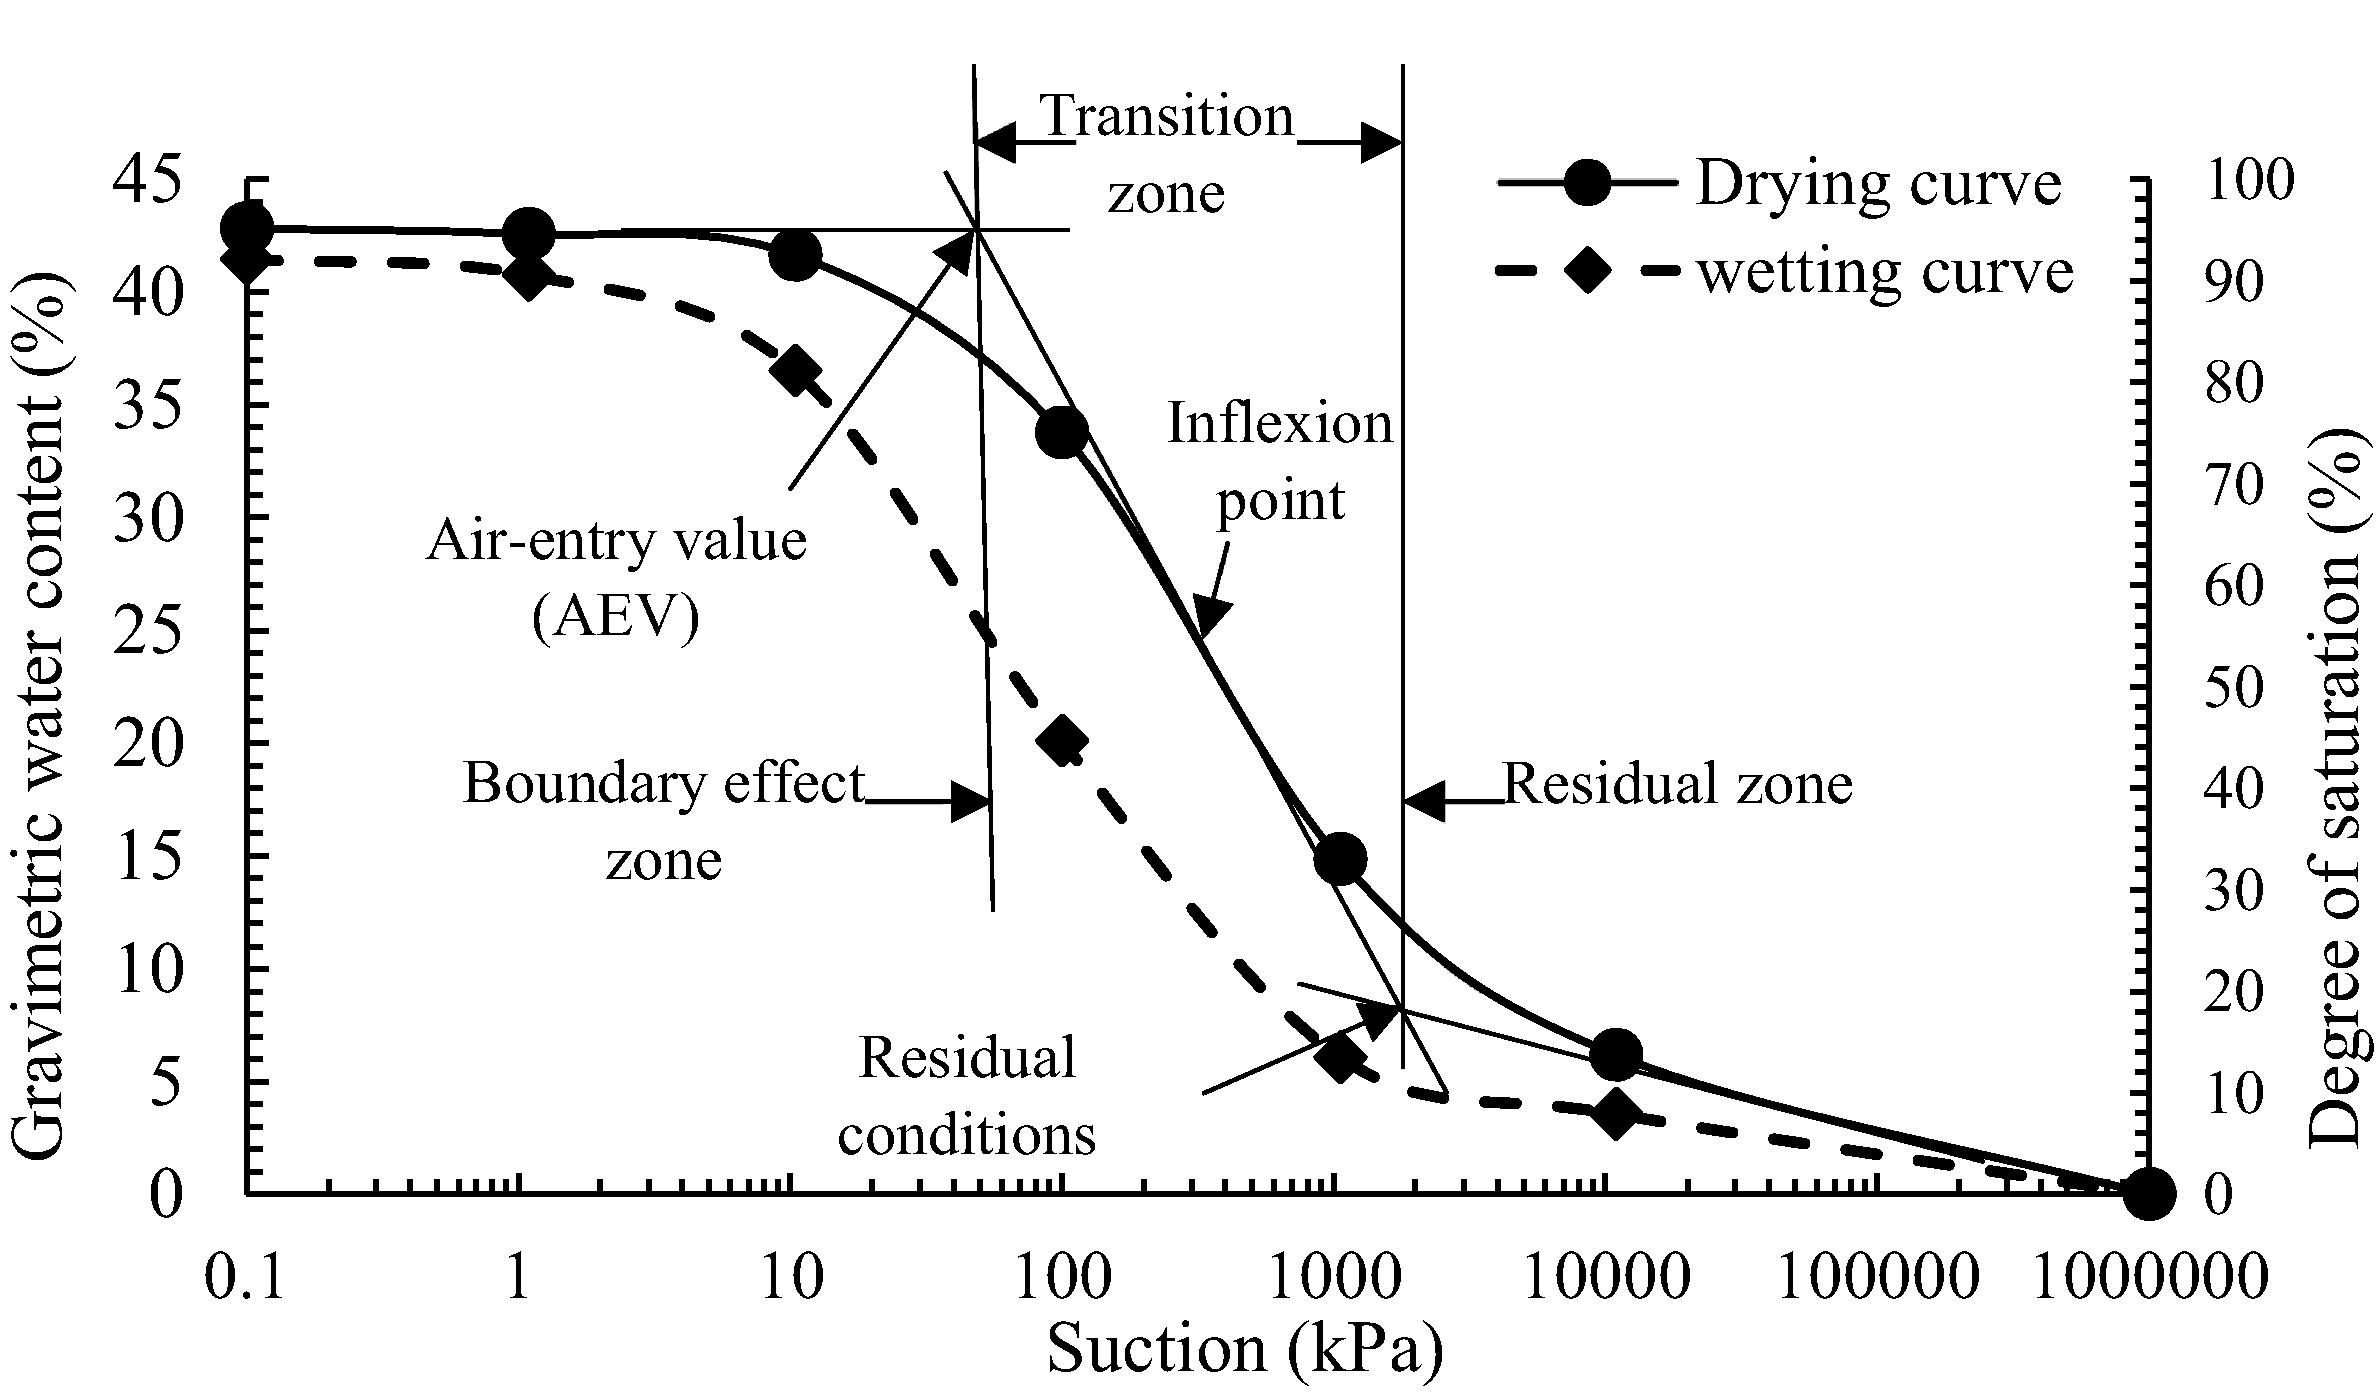
\includegraphics[width=0.8\textwidth]{gfx/chapter-data-analysis/swcc.jpg}
	\caption[Example SWCC.]{Example SWCC (\cite{Eyo2020}).}
	\label{fig:swcc-example}
\end{figure}

\section{Data and Modeling}
Data collected was 5 minute averages of 1 minute records (values were measured every minute and stored every 5 minutes as the average of the previous 5 values) over the course of the 3 year study (May 2017 - November 2020).
This data resolution captures enough detail without producing an overwhelming number of data records.
To better synthesize the data collected, summary statistics for predefined hydrological events are generated based on either a total amount of rainfall followed by a minimum dry time (typically 6 hours), or based on characteristics of other variables of interest, namely ponding and soil moisture values.

\subsection{Rainfall Events}
Using clearly defined rules to identify events is the first step to generating meaningful summary statistics that are applicable across time and space, and useful for comparing GSI with dissimilar properties.
In a GSI context, events are storms that result in a measurable quantity of precipitation.
Small events typically do not have a pronounced impact on GSI, but the effectiveness of GSI systems is typically greater for smaller or less intense storm events (\cite{Liu2020}).
However, these smaller events make up the bulk of storm events observed at SMP A and by others (\cite{Albright2018}), with 95\%\ of observed total rainfall less than 42mm (Figure \ref{fig:event-total-rainfall}).
For this analysis, a `standard,' or `normal' storm event begins when rainfall is first recorded and continues until 6 hours after the last observed rainfall, as studies have shown storms separated by 6 or more hours to be meteorologically separate events (\cite{Wadzuk2017}).
This means the minimum event duration is 6 hours, and any periods without rainfall of less than 6 hours are continuations of the same storm event.
This definition is used as the standard both for generating storm summary data in monthly reports to PennDOT and for all analyses henceforth that do not directly involve soil moisture observations.
During the period of interest, there were 414 observed standard events with a mean duration of 12.2 hours, a median of 9.5 hours, and a standard deviation of 7.5 hours. The data are highly right-skewed, with a maximum of 52.2 hours, and appear to follow a roughly chi-square distribution (Figure \ref{fig:event-duration-histogram}).

\begin{figure}[ht]
	\centering
	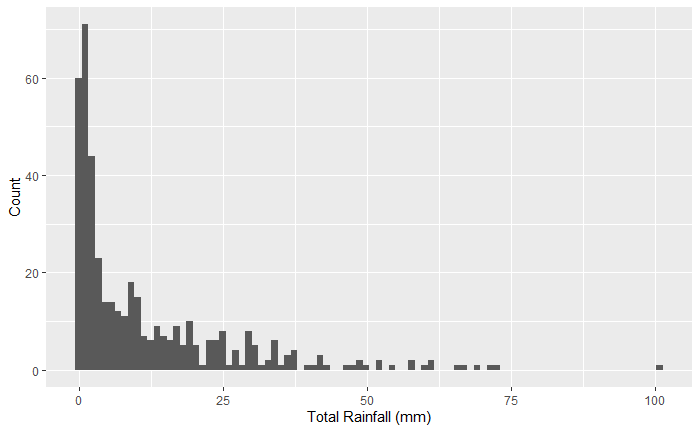
\includegraphics[width=\textwidth]{gfx/chapter-data-analysis/hist_rainfall_depth.png}
	\caption{Distribution of event total rainfall depths.}
	\label{fig:event-total-rainfall}
\end{figure}

\begin{figure}[ht]
	\centering
	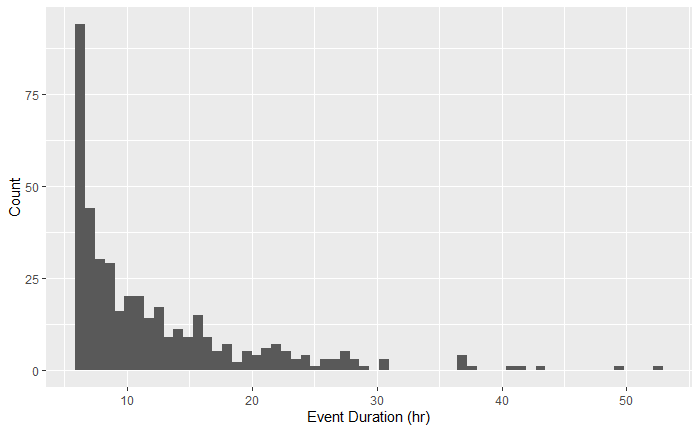
\includegraphics[width=\textwidth]{gfx/chapter-data-analysis/hist_duration.png}
	\caption{Distribution of event lengths.}
	\label{fig:event-duration-histogram}
\end{figure}

Events are distributed throughout a Gregorian 365-day year approximately uniformly, as seen in Figure \ref{fig:event-date-histogram}, although there are some notable event clusters in both late spring (around ordinal day 150), and during hurricane season (after ordinal day 200).
There are notably fewer events during the winter months, but this is likely due to the instrumentation's lack of sensitivity to snowfall.
Snowfall events are also less taxing on GSI systems in general, although snowmelt events may have similar characteristics to a rainfall event but have not been studied.

\begin{figure}[ht]
	\centering
	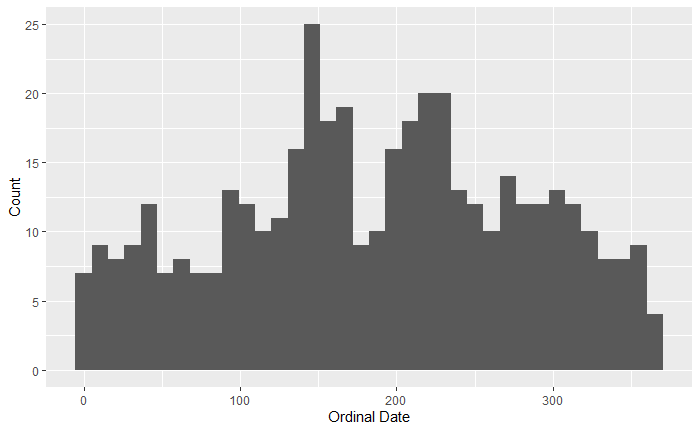
\includegraphics[width=\textwidth]{gfx/chapter-data-analysis/hist_ordinal_date_event.png}
	\caption{Distribution of event ordinal dates.}
	\label{fig:event-date-histogram}
\end{figure}

\subsection{Soil Moisture Events}
Events involving soil moisture require a modified approach to event definition due to the prolonged nature of soil moisture's response to storm events.
Soil moisture, and by extension ponded water atop saturated soils, take longer than 6 hours to recover after storms of interest.
Studies have shown that the recovery period for soils is 72-96 hours (\cite{Davis2009,Wadzuk2017}).
To define events for these analyses, both rainfall and soil moisture levels are considered.
As before, an event begins with the first observed rainfall.
However, the end of the event is defined by a user-defined minimum event time (6 hour default) as well as a threshold ponding level or soil moisture level (either may be used, depending on the type of analysis being performed).
A simple moving average of the number of steps comprising the minimum event duration (in other words, the data interval - 5 minutes - divided into the minimum event time of interest) provides a window into the past or the future at a given time step, and can be used to define an event as follows:
\begin{equation}
	\begin{aligned}
		\centering
		Event = & \{ A = [ moving\_average(rainfall, Q / P) > 0 ], \\
				& B = [ moving\_average(rainfall, Q / P) == 0 \\
				& \cap moving\_average(K, Q / P) < R ] \}
	\end{aligned}
	\label{eq:alt-event-definition}
\end{equation}
where A is an indicator for the beginning of an event, B is an indicator for the end of an event, Q is the minimum event duration, P is the observation interval, R is a threshold value, and K is the variable of interest.
Timestamps falling between successive A and B values are assigned a unique, random string of eight characters generated from the first timestamp in the series.
The distribution of these specialized events is similar to that of the standard events above, although there are fewer (214) of them due to the increased length of events capturing a greater share of rainfall per event.

\section{Key Performance Indicator Definitions}

\subsection{Recession Rate}

Calculating a water level differential across consecutive data records can be used to determine periods of increasing or decreasing volume in the ponded storage.
Recession of the pond is indicated by a negative change in level, although no rainfall or inflow can happen simultaneously to ensure that change in level is solely due to outflow from the system (i.e., infiltration or overflow).
Additionally, if the recession rate due to only infiltration is desired, the water level must be below the overflow point of any outlet structures.
The magnitude of recession is directly correlated to infiltration rate, which is governed by the type and health of the GSI soils (\cite{Gregory2006, Horton1994}).
Larger recession rates indicate a faster drawdown of the water level, while smaller values could be due to prolonged saturation conditions or under-performance due to compaction or clogging of soil pores.
Comparing average recession rates calculated over the duration of a storm to other simultaneously recorded atmospheric (temperature, relative humidity, barometric pressure) and GSI state (current pond level) data shows the relationships that have the most significant impact on GSI performance.
Changes in the recession rate over the period of a storm or over long periods of time (e.g., seasonal, annual, etc.) indicate changes in the soil health (\cite{Jenkins2010,Zukowski2016}).

The relationships between recession and atmospheric variables or GSI state are complicated by several factors, namely the timing and size of an event, the pre-event geomorphology and hydrologic state of the GSI, and their collective interaction.
The timing and size of a storm event, which can be best described by a combination of time of year, hyetograph, and the length of time since the previous storm event, are important because these play the largest role in determining the GSI pre-storm state's response to specific storm conditions.
A GSI system will respond differently at different times of the year to two events with identical hyetographs, while the same GSI with identical starting conditions will respond differently to two different hyetographs (\cite{Braga2007,Joshi2019}).
Varying any single variable used to describe an event changes the GSI system's initial response to that event.

The variability of the pre-event state of the GSI necessitates an adaptable baseline to use in evaluating performance.
Performance cannot simply be stated as the change from pre-event conditions because this would make comparisons between dissimilar pre-event states unnecessarily complex.
For example, a storm taking place during early spring in the Philadelphia, PA region could have a wide range of pre-storm soil moisture, air and water temperatures, or plant growth conditions, to name a few, all of which will impact how the system responds at the beginning of a storm.
Additionally, the fact that suction head is highest when the soil is dry (\cite{Eyo2020}, Figure \ref{fig:swcc-example}), means that infiltration loss is greatest at the beginning of an event, no matter the specific initial conditions, because that is when the soil is driest.
This inverse relationship indicates that the most consistent method of comparison will be when the system reaches equilibrium and is treating water at a constant rate.
For recession rates, this means looking at the trailing end of a storm, when inflow has ceased, ponding level has reached its peak, and the soil has reached saturation.
Examining the end of a storm removes the influence of a specific storm event's timing characteristics and focuses the performance evaluation on how the system reduces ponded volume and recovers from saturation.
Full infiltration of ponded water is required within 72 hours in Philadelphia.
Observations show that the majority of storms have complete infiltration of the ponded water within 6 hours post-rainfall.

\subsection{Infiltration Drying Rate}
The recession of water within the soil column also reflects the soil health of the site.
Using soil moisture probes at 10, 35, and 60 cm allows the calculation of an average rate of the descent of saturation conditions, or `drying front', as the soil capacity recovers.
This subsurface drying rate should remain consistent between events of different sizes (\cite{Wadzuk2017}), provided the soils reach saturation prior to the end of measurable ponding.
Soil moisture values during a storm event typically produce a curve like that in Figure \ref{fig:typ-soil-moisture}.
The soil moisture curve tends to respond with a sharp upward jump, 5-20 minutes in length, at the beginning of the storm event's inflow when the wetting front passes each sensor and soil approaches full saturation.
This increase in saturation coincides with a sharp drop in suction head, as the soil's ability to pull water in quickly is greatly reduced once saturated.
The soil moisture curve has been characterized with a series of seven points in work completed by Matina Shakya, a Ph.D. Candidate working on soil moisture measurements for VCRWS/PennDOT.
The beginning and end of this increase in soil moisture at the inflow onset are identified as points A and B, respectively.
Point A is typically below 0.40, or 40\% volumetric water content (VWC), while points B and C are typically between 0.45 and 0.50, or 45-50\% VWC.
Soil moisture levels remain at saturation conditions for the duration of ponding, due to continuous infiltration.
The reduction in volume from the system due to evaporation, evapotranspiration, or any other means is assumed to be negligible compared to infiltration during a storm and in the hours immediately after.
When ponding has ended, infiltration continues as the saturated zone recedes down into the soil profile (Figure \ref{fig:drying-rate-sketch}).
The trailing limb of the saturation curve can be identified by two additional points, C and D (Figure \ref{fig:typ-soil-moisture}), identified as the drop off point and inflection point of the soil moisture curve, respectively.
In Figure \ref{fig:drying-rate-sketch}, the difference in time between steps 2 and 3 at each sensor depth (10, 35, 60cm) is the subject of interest.

\begin{figure}[ht]
	\centering
	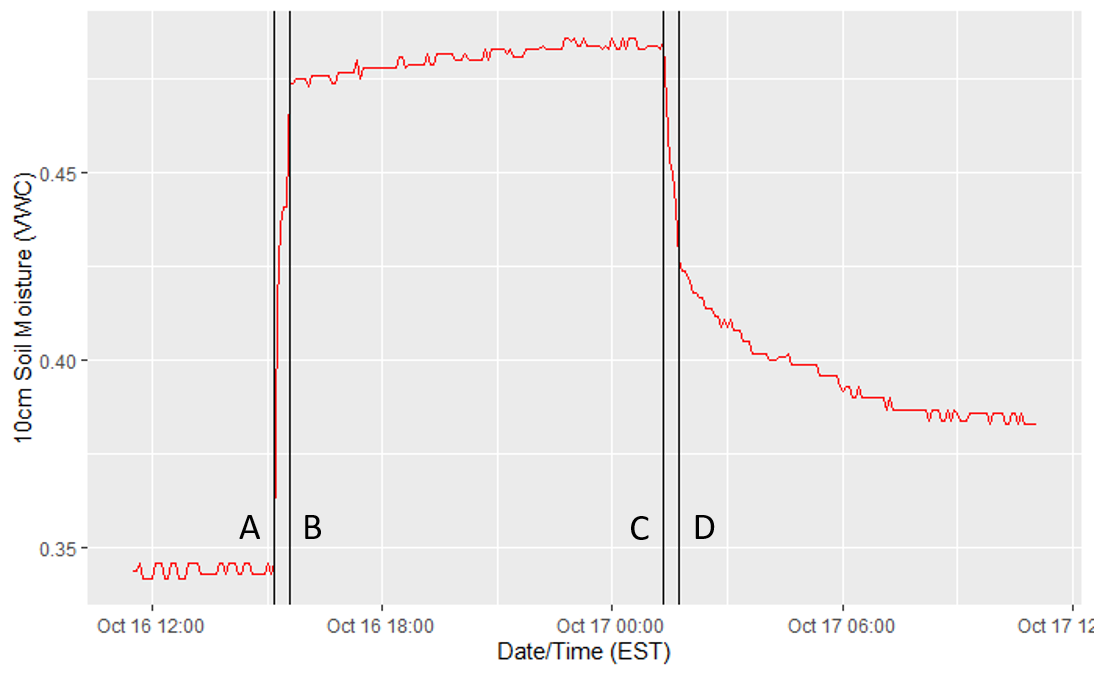
\includegraphics[width=\textwidth]{gfx/chapter-data-analysis/typ_soil_moisture.png}
	\caption[Typical soil moisture curve.]{Typical soil moisture curve. Vertical black lines denote points A, B, C, and D from left to right, respectively.}
	\label{fig:typ-soil-moisture}
\end{figure}


\begin{figure}[ht]
	\centering
	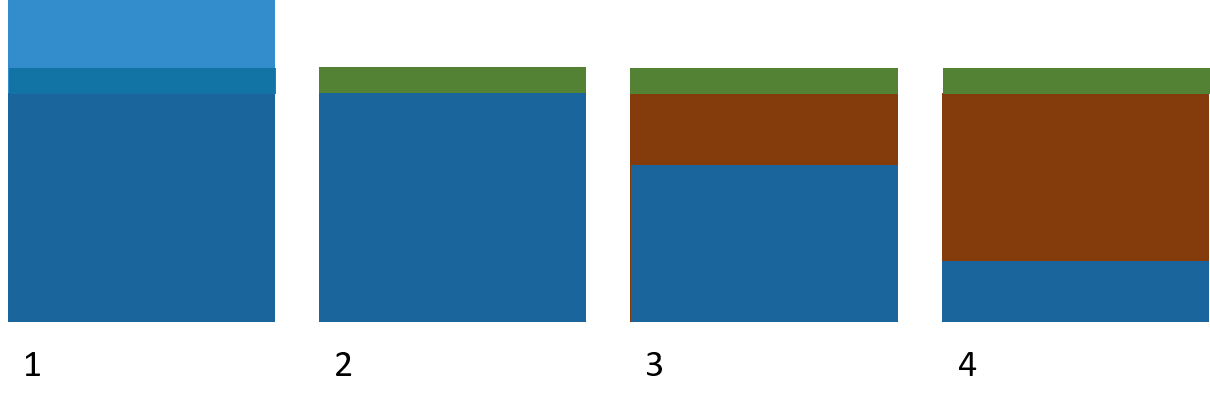
\includegraphics[width=\textwidth]{gfx/chapter-data-analysis/drying_rate_sketch.png}
	\caption[Illustration of infiltration drying rate.]{Illustration of infiltration drying rate showing 1. ponded water, 2. end of ponding, 3. top-most soil returns to field capacity, 4. saturation zone reaches equilibrium with water table.}
	\label{fig:drying-rate-sketch}
\end{figure}

The calculation of this metric is slightly more complicated than raw recession rate of the ponded water presented earlier.
The inflection points A, B, C, and D are calculated as the four primary peaks in the absolute value of the first differential of the soil moisture data:

\begin{equation}
	\centering
	Inflection Point\{A,B,C,D\} = local max(|\theta_{i} - \theta_{i-1}|)_{j}
	\label{eq:soil-moisture-inflection}
\end{equation}

where i = {1,2...n} for n soil moisture observations ($\theta$) in a given storm and where j = {1,2,3,4} corresponding to {A,B,C,D}.
These points are easily calculated using the `findpeaks' function from the R package `pracma' (\verb+pracma::findpeaks(...)+).
The function takes a vector of data, the absolute value of the differential soil moisture data applicable to one storm event in this case and returns the ordered indices of the requested number of local maximums (four in this case).
Depending on the specific values of soil moisture seen during an event, the four indices may be returned in any order, largely based on the magnitude of difference between any two given points, so the resulting points are sorted and assigned to A through D respectively.
However, due to the highly variable pre-event state of the GSI, storm events that begin with saturated VWC values (>0.44 VWC) often misidentify some or all of these points, so these events have been disregarded in the context of this analysis.

\section{Results and Discussion}

\subsection{Recession Rate}

\subsubsection{Temperature Dependence}
The weather station at SMP A records air temperature, and each pressure transducer (PT) records the temperature of surrounding water.
The two types of temperature are highly correlated (Pearson correlation = 0.981).
This analysis only considers water temperature since the water is in direct contact with the soil and displays some variance of viscosity at different temperatures.
Testing for variations in recession rate across the range of observed water temperatures shows a linear relationship (Figure \ref{fig:temp-vs-recession-by-storm}), as evidenced by the high correlation coefficient of 0.735 and $R^2$ of 0.54.

\begin{figure}[ht]
	\centering
	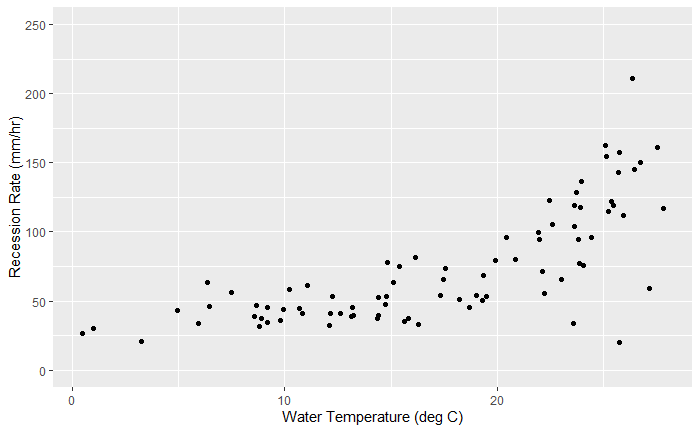
\includegraphics[width=\textwidth]{gfx/chapter-data-analysis/temperature_vs_recession_rate_by_storm.png}
	\caption{Average water temperature vs recession rate for SMP A storm event.}
	\label{fig:temp-vs-recession-by-storm}
\end{figure}

The relationship between recession rate and ponded water temperature becomes more apparent when temperature is separated into similar temperature range bins (Figure \ref{fig:temp-vs-recession-binned}).
Five bins were chosen to ensure the number of events per bin was at least 10 for most bins.
The trend of higher observed recession rates at higher temperatures is clear.
The lowest bin ((-0.05,5.83]) has only seven events but follows an identical trend to the upper four bins in magnitude of mean and quartiles (indicated by upper and lower vertical lines).
This trend aligns with several physical and hydrologic models, namely that warmer water is less viscous and flows easier, especially through the soil (\cite{Emerson2008}).
This finding means that GSI performance can be expected to increase during warmer months, both due to increased infiltration capacity and increased water uptake and evapotranspiration by the plant mass (\cite{Bartens2008}).
Furthermore, it has been shown that soils that have experienced multiple freeze-thaw cycles have higher values of saturated hydraulic conductivity due to the formation of internal ice crystal structures within frozen soils, which can expand pore space and increase the "development of macroscopic cracks and microscopic voids" (\cite{Asare1999}).
Therefore, soils that experience freezing conditions followed by warm conditions, as is typical in a climate with a distinct harsh winter season, can expect to see a natural "loosening" of the soil via the creation of these additional void spaces.
This increase in void spaces has the potential to cause preferential flow paths through the soil, which will lead to increased infiltration rates up to the frost line.

\begin{figure}[ht]
	\centering
	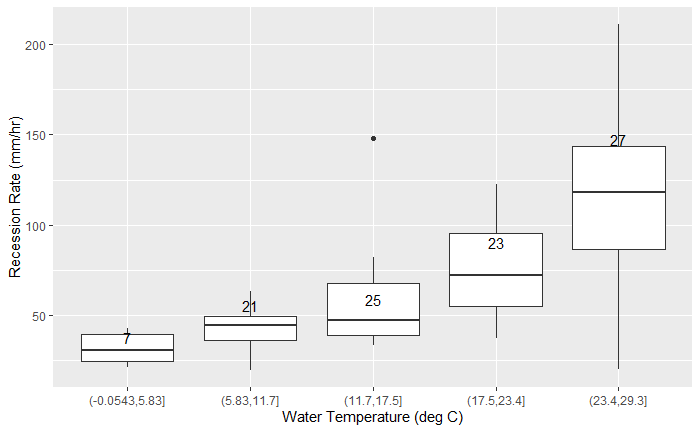
\includegraphics[width=\textwidth]{gfx/chapter-data-analysis/temperature_vs_recession_rate_binned.png}
	\caption[Average water temperature vs recession rate.]{Average water temperature vs recession rate, separated into bins, with the number of storm events per bin indicated.}
	\label{fig:temp-vs-recession-binned}
\end{figure}

\subsubsection{Insignificant Relationships}
Both relative humidity (RH) and barometric pressure, recorded in a similar fashion to air temperature at SMP A, showed no significant relationship with recession rate, with correlation coefficients of 0.148 and 0.25 and $R^2$ values of 0.022 and 0.064 respectively.
Comparing the average recession rate to RH bins and pressure bins shows no correlation between different values for these variables as compared to the average recession rate (Figure \ref{fig:recession-rh-bin} and \ref{fig:recession-pressure-bin}).

\begin{figure}[ht]
	\centering
	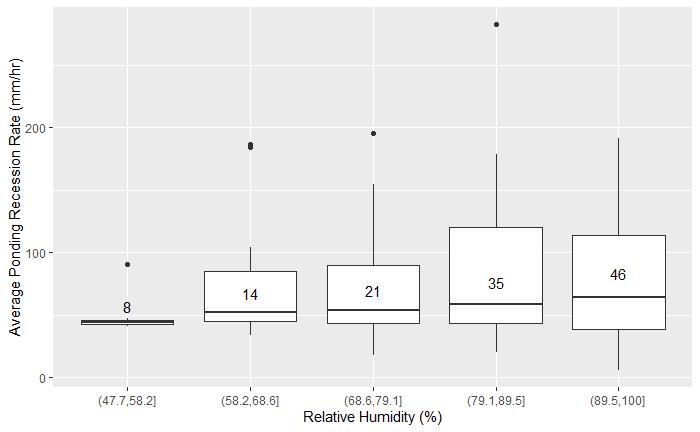
\includegraphics[width=\textwidth]{gfx/chapter-data-analysis/rh_vs_recession_rate_binned.png}
	\caption{Average Relative Humidity vs Recession Rate.}
	\label{fig:recession-rh-bin}
\end{figure}

\begin{figure}[ht]
	\centering
	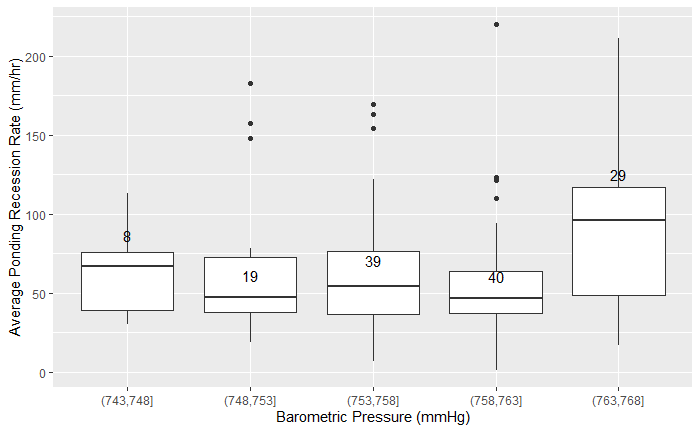
\includegraphics[width=\textwidth]{gfx/chapter-data-analysis/pressure_vs_recession_rate_binned.png}
	\caption{Average Barometric Pressure vs Recession Rate.}
	\label{fig:recession-pressure-bin}
\end{figure}

From these observations, GSI performance is not dependent on barometric pressure or relative humidity, which largely only impact the soil-air interface.
The lack of relationship between the atmosphere and sub-surface infiltration mechanics is expected, since the soil contains enough mass to prevent significant influence from the relatively fast-changing atmosphere.

The level of ponded water collected in the rain garden similarly has no significant effect on the rate of recession, with a correlation of -0.2 and $R^2$ of 0.043.
This runs contrary to expectations that greater head pressure at the soil-ponding interface would lead to higher recession rates.
The rate of recession is consistent across nearly the entire ponding depth range (Figure \ref{fig:recession-ponding-depth-bin}).
\begin{figure}[ht]
	\centering
	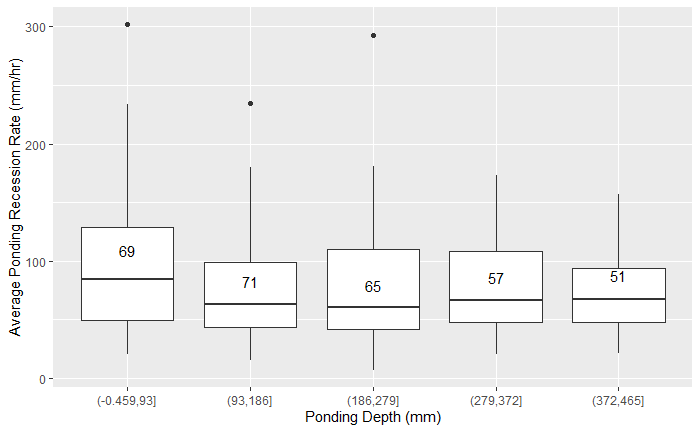
\includegraphics[width=\textwidth]{gfx/chapter-data-analysis/pond_depth_vs_recession_rate_by_storm.png}
	\caption{Average Ponding Depth vs Recession Rate.}
	\label{fig:recession-ponding-depth-bin}
\end{figure}
The lack of correlation, while surprising, could be due to the fact that sub-surface saturation leads to high enough pore water pressure such that it cancels out the head pressure seen at typical ponding depths of up to a maximum of less than 1 meter.
Additionally, the shallow profile of the garden bed means that a depth measurement taken in the middle of the garden captures the deepest point, and less significant depths are experienced by the majority of the surface area (\cite{Sokolovskaya2021}).
While the slope estimate and F-statistic in a linear model for recession rate and pond depth are both significant at the 0.05 level, the low $R^2$ value means the model is only predicting the mean recession rate.


\subsubsection{Regression}
Using multiple linear regression, a numeric relationship between the recession rate and pond temperature, max pond depth, ponding duration, total rainfall, and average rainfall intensity can be determined.
The expected value of this relationship can determine if a GSI system is functioning nominally.
Values that are outside the expected relationship boundaries are a cause for concern, and a trend of values outside the norm would indicate that maintenance or further evaluation of the system is required.
While the numbers presented here are specific to PennDOT's SMP A, this approach, and indeed the entire scope of data collection, storage, and analysis would be of tremendous value to any system or group of systems with similar properties.

Regressing the following parameters onto ponding recession rate (mm/hr) results in the listed effects (Table \ref{table:pond-recession-regression}), which results in Equation \ref{eq:pond-recession-regression}.
The R-squared value is 0.9023, with an F-statistic (significance test) of 312.1 on 5 and 169 degrees of freedom (p-value = $<2.2e-16$), indicating the partial slopes ($\beta_1\dots\beta_5$) are not equal to 0.
There are, however, normality concerns, as demonstrated by the normal quantile-quantile plot (Figure \ref{fig:pond-recession-regression-normal-qq}), which shows a departure from linearity beyond $\pm1.5$ quantiles, suggesting that there have been a number of extreme observations.
This is expected, as the data are not normally distributed, so an additional nonparametric test is required to confirm the trend seen.
The relationship lacks an intercept because the mean response is expected to be 0 mm/hr, corresponding to no ponding recession when all other variables are also 0.

\begin{table}[ht!]
\centering
\caption{Ponding recession rate regression results.}
	\begin{tabular}{|l|l|l|l|l|l|}
		\hline
		& Coefficient & Estimate & Std. Error & t value & Pr($>|t|$) \\
		\hline
		$\beta_{1}$ & B1 pond mean temp (\degree C)  & -0.238 & 0.085 & -2.801 & 0.005697 \\
		$\beta_{2}$ & B1 pond max depth (mm)         & -0.117 & 0.006 &-20.622 & $<$2e-16 \\
		$\beta_{3}$ & B1 ponding duration (hr)       &  0.981 & 0.225 &  4.361 & 2.24e-05 \\
		$\beta_{4}$ & Total Rainfall (mm)            &  0.182 & 0.064 &  2.846 & 0.004980 \\
		$\beta_{5}$ & Average Intensity (mm/hr)      & -0.377 & 0.110 & -3.416 & 0.000797 \\
		\hline
	\end{tabular}
\label{table:pond-recession-regression}
\end{table}

\begin{equation}
	\centering
	y = - \beta_1 * 0.2384 - \beta_2 * 0.11721 + \beta_3 * 0.98104 + \beta_4 * 0.1821 - \beta_5 * 0.3771
	\label{eq:pond-recession-regression}
\end{equation}

\begin{figure}[ht!]
	\centering
	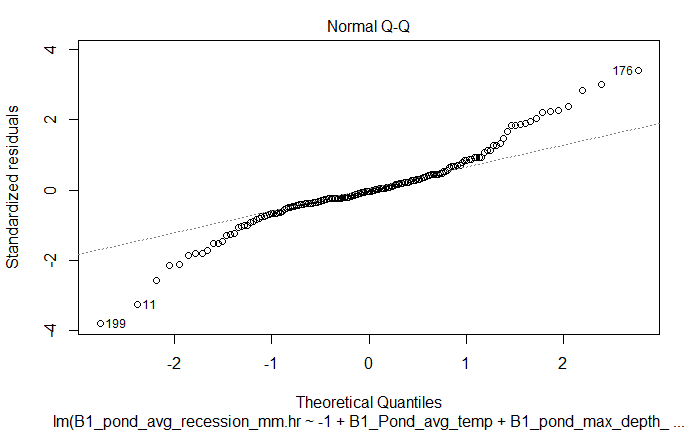
\includegraphics[width=\textwidth]{gfx/chapter-data-analysis/pond_recession_regression_normal_qq.png}
	\caption{Normal Q-Q plot for ponding recession regression.}
	\label{fig:pond-recession-regression-normal-qq}
\end{figure}

The regression model in Equation \ref{eq:pond-recession-regression} was chosen for its high R-squared value, which reflects the percent of variation in the response (recession rate) explained by the total variation in the model parameters, as well as its overall significance (high F-statistic with low p-value).
Parameters kept in the model (listed in Table \ref{table:pond-recession-regression}) have individual p-values < 0.05.
Estimates of recession rate predict the mean response for each unit change of the model parameters multiplied by their respective coefficients.
Other models considered included some combination of the final parameters, water temperature, event duration, and ordinal day.
While the equation predicts the mean response given a set of inputs and will not always be precise, a confidence interval of 95\%\ can indicate values that are outside the expected range.
Consecutive events with abnormally high or low recession values will indicate a need for inspection or intervention.

The model is not without its shortcomings, however, and does not account for departures from normality of the training data.
The Kendall seasonal trend statistic, $\tau$, tests for seasonal trends in monotonic, nonparametric data.
The $\tau$ statistic is a ratio of the probabilities of the observed order of the data to that of a different ordering.
That is, assuming two variables (X and Y, for example) are independent, the expected value of $\tau$ is 0, as the likelihood of the observed ordering is equal to that of any other ordering for two independent series \cite{Abdi2007}.
Calculating $\tau$ for comparison between B1 recession rate and the variables found in the regression equation \ref{eq:pond-recession-regression} results in the values found in Table \ref{table:kendall-test-results}.
All the relationships are significant enough to reject the claim that the pairwise comparisons are independent, suggesting the trends observed, and by extension their inclusion in a normal multiple regression, are significant, despite the lack of normality.

\begin{table}[ht!]
	\centering
	\caption{Kendall seasonal trend results.}
	\begin{tabular}{|l|l|l|}
		\hline
		Variable & Kendall $\tau$ & p-value \\
		\hline
		B1 pond mean temp (\degree C) & 0.122 & 0.001711 \\
		B1 pond max depth (mm)        & 0.915 & $<$2.2e-16 \\
		B1 ponding duration (hr)      & 0.829 & $<$2.2e-16 \\
		Total Rainfall (mm)           & 0.548 & $<$2.2e-16 \\
		Average Intensity (mm/hr)     & 0.410 & $<$2.2e-16 \\
		\hline
	\end{tabular}
	\label{table:kendall-test-results}
\end{table}

\subsection{Infiltration Drying Rate}

There are 76 valid events during the period of interest, essentially a subset of the standard events, quantified with different ending criteria to focus on soil moisture recovery.
For each event, the rate of drying for the three zones between the surface and the three soil moisture sensors at progressively deeper placements is calculated as distance/time.
Figures \ref{fig:drying-rate-pond-10}, \ref{fig:drying-rate-10-35}, and \ref{fig:drying-rate-35-60} demonstrate that this rate can be expected to fall within 0-5 cm per hour.
The 95\% percentile falls at 9.5 hours between 10 and 35cm (approx 2.63cm/hr), and 7.4 hours between 35 and 60cm (approx. 3.37cm/hr), meaning 95\% of events can be expected to exhibit drying rates faster than this.
The distribution does not display correlation with water temperature (Pearson correlation 0.047, p-value 0.34), and has remained consistent over time, as displayed in Figure \ref{fig:drying-rate-vs-time}.

The infiltration drying rate compares favorably to Saturo constant-head infiltration testing performed at the site across three growing seasons (repeat tests performed in downstream and upstream basins at discrete locations).
These tests showed a mean $K_{sat}$ value of 1.3-6.2 cm/hour, which compares favorably with the mean infiltration drying rate of 1.8-9.5 cm/hour.
Both metrics have large variances, and it would be helpful to do more direct comparison testing to investigate if the variability is consistent between them.

\section{Conclusions}
The methods described here attempt to evaluate methods for comparing storm events across time and space.
Using recession and infiltration KPIs to evaluate a system of GSI performance across an entire region will enable insights into long term design successes, and early detection of system errors.
The data have shown that performance is most highly impacted by temperature, which oscillates with an annual seasonal period.
GSI health can generally be quantified in terms of recession and drying rates for ponding level and soil moisture, respectively.
Higher rates for each quantify indicate faster transfer of water into the subterranean water table, and faster reduction in soil moisture that will lead to quicker preparation for the next storm.

In general, average recession rates between 40 and 120 mm/hr can be expected, depending on time of year and water temperature.
Average drying rates as high as 9.5 cm/hr can be expected, although this value would be expected to vary from GSI to GSI based on soil design criteria.
These statistics are not dependent on GSI parameters such as surface area, loading ratio, or number of inlets or outlets, and are therefore independent of site configuration.
The statistics can be calculated for any GSI system, or part of a system, to determine if infiltration rates and recovery rates fall within the expected range.
Thanks to the few parameters needed, namely ponding depth and soil moisture level, few sensors are necessary, keeping costs for this kind of monitoring low, making it accessible to be deployed at a larger number of sites, or at multiple locations within a single site.
While this work intentionally does not address spatial variability within a single site for infiltration or drying rates, the data collected are assumed to represent the average conditions throughout SMP~A, and the same assumption would be valid for the statistics calculated at other sites in a similar manner.

The recession and infiltration rates are affected by conditions both above and below the soil surface and provide an acceptable proxy for soil health.
The recession rate is shown to be affected by temperature and could be reduced by clogging of the soil surface or compaction of lower soil layers, leading to reduced rates.
Similarly, the infiltration drying rate is shown to be consistent across a wide variety of GSI conditions and could be adversely affected by changing soil properties that make the GSI function less efficiently.
The established relationships and expected values for each are useful as indicators for long term performance, and departures from expectations are cause for further investigation.

\begin{figure}[ht!]
	\centering
	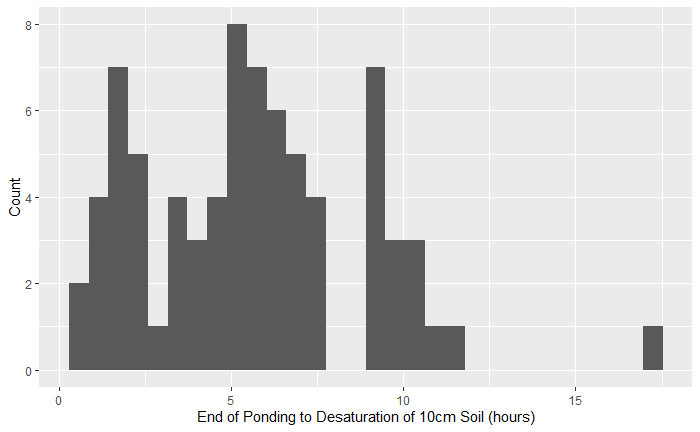
\includegraphics[width=\textwidth]{gfx/chapter-data-analysis/drying_rate_pond_10.png}
	\caption{Time to Desaturation from end of ponding to 10cm.}
	\label{fig:drying-rate-pond-10}
\end{figure}

\begin{figure}[ht!]
	\centering
	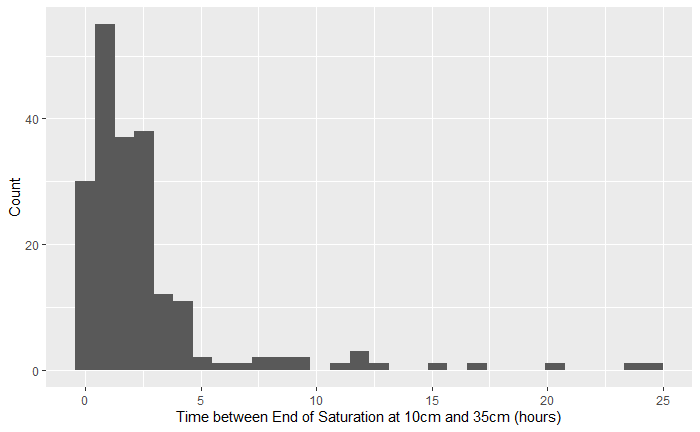
\includegraphics[width=\textwidth]{gfx/chapter-data-analysis/drying_rate_10_35.png}
	\caption{Time to Desaturation from 10 to 35cm.}
	\label{fig:drying-rate-10-35}
\end{figure}

\begin{figure}[ht!]
	\centering
	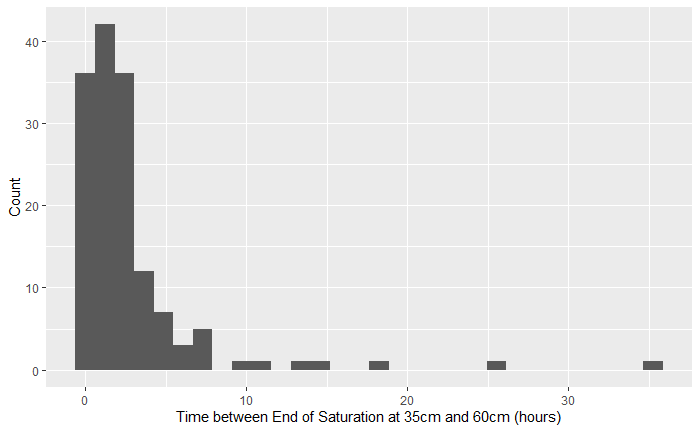
\includegraphics[width=\textwidth]{gfx/chapter-data-analysis/drying_rate_35_60.png}
	\caption{Time to Desaturation from 35 to 60cm.}
	\label{fig:drying-rate-35-60}
\end{figure}

\begin{figure}[ht]
	\centering
	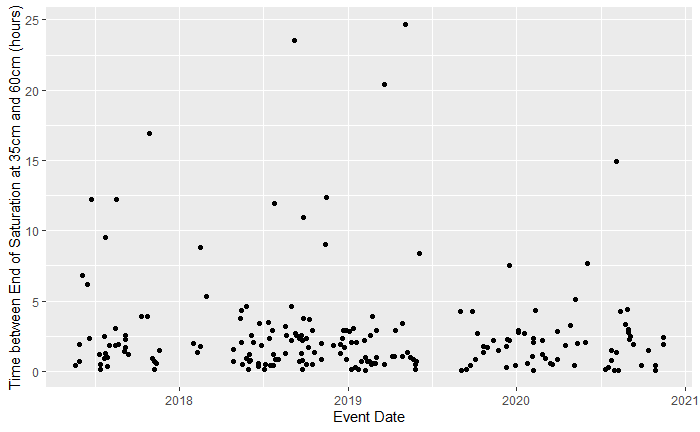
\includegraphics[width=\textwidth]{gfx/chapter-data-analysis/time_vs_drying_rate_10_35.png}
	\caption{Event Date vs Time to Desaturation from 10 to 35cm.}
	\label{fig:drying-rate-vs-time}
\end{figure}